% !TeX root = ../ejemplo.tex

\section{Reconocimiento facial}

El reconocimiento facial es una técnica que permite a las computadoras predecir la identidad de una persona desde una imagen \cite{L14}.

Tiene múltiples aplicaciones en la industria como el desarrollo de sistemas de asistencia, en la salud, sistemas de seguridad, etc \cite{L15}. 

\subsection{Pipeline de un sistema moderno de reconocimiento facial}

A menudo, los términos verificación de rostros e identificación de rostros se usan de forma indistinta, sin embargo, aunque ambos comparten el mismo dominio del problema, lo abordan de forma distinta \cite{L16}.

Para entender mejor la diferencia entre ambas tareas y su papel en el desarrollo de un sistema de reconocimiento facial, explicaremos como los sistemas modernos de reconocimiento facial operan a través de una secuencia de etapas bien definidas, donde cada una es indispensable para obtener resultados precisos y fiables \cite{L15}.\\

En cualquier pipeline, la interdependencia entre sus etapas es crucial, ya que la calidad y el éxito de cada fase dependen directamente del desempeño de la anterior. Un ejemplo claro es la etapa de detección de rostros: los modelos de extracción de características esperan recibir una imagen de un rostro correctamente identificada. Si se emplean técnicas de detección poco robustas, el módulo siguiente puede fallar en la extracción de características, lo que resulta en una menor precisión en los resultados finales \cite{Face_OpenCV}.\\

Por lo tanto, a continuación se presentan las etapas fundamentales de un sistema de reconocimiento facial actual:

\begin{figure}[htbp]
	\begin{center}
		\fbox{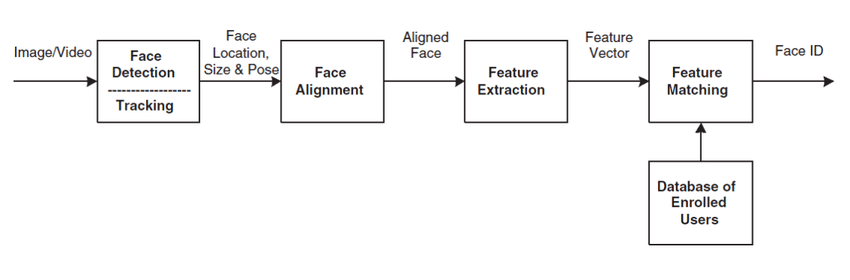
\includegraphics[width=.68\textwidth]{images/face_pipeline}}
		\caption{Pipeline moderno de un sistema de reconocimiento facial.}
		\label{fig:Pipeline de un sistema de reconocimiento facial}
	\end{center}
\end{figure}


\subsubsection{Detección de rostros}

Esta es la etapa inicial, donde el sistema identifica la presencia de rostros en una imagen o video y determina su ubicación, generalmente mediante el cálculo de cuadros delimitadores. Se emplean modelos especializados que no solo identifican los cuadros delimitadores, sino que también detectan puntos clave faciales (como ojos, nariz y boca), los cuales son esenciales para la alineación posterior \cite{L16}.\\

Algunos algoritmos y técnicas empleadas en este punto incluyen métodos tradicionales como el algoritmo Viola Jones o implementaciones más recientes basadas en aprendizaje profundo como MTCNN o RetinaFace \cite{L14}.\\

Como se mencionó, este paso es la base del sistema de reconocimiento facial, por lo que su correcta implementación puede repercutir drásticamente en los resultados obtenidos.\\


\subsubsection{Alineación de rostros}

Una vez detectados, los rostros se estandarizan en orientación y tamaño utilizando los puntos clave extraídos. Este proceso implica rotar, escalar y recortar los rostros para asegurar que características como los ojos y la boca estén posicionadas de manera consistente \cite{Face_OpenCV}.\\

El propósito de la alineación es reducir las variaciones causadas por la pose o la inclinación, haciendo que las entradas sean más uniformes para las etapas posteriores y asegurando que el modelo de embedding se enfoque en las características relevantes, lo que mejora la calidad y fiabilidad de los embeddings \cite{L16}.\\

Se ha demostrado que, la alineación de rostros mejora la precisión obtenida por este tipo de sistemas \cite{Face_OpenCV}.

\subsubsection{Extracción de características o representación en forma de embeddings}

Una vez que las imágenes de los rostros se encuentran correctamente procesadas, es decir, se identificaron y recortaron los rostros, seguidos de una alineación, se procede a usar algún modelo para la generación de embeddings como \textit{FaceNet o ArcFace} los cuales generan vectores de alta dimensionalidad \cite{Face_OpenCV}.\\

El propósito de esta etapa es transformar los datos complejos de una imagen en un formato numérico, compacto y sobre todo, comparable para lograr una eficiente comparación en el siguiente punto \cite{L16}.


\subsubsection{Identificación o verificación de rostro}

Los embeddings faciales obtenidos se comparan con una base de datos utilizando medidas de similitud como la distancia coseno o euclidiana. Este paso permite determinar si dos rostros corresponden a la misma persona (verificación) o identificar a una persona entre múltiples registros (identificación) \cite{L14}.



\subsection{Identificación de rostros}

Como ya se mencionó, la identificación de rostros y la verificación de rostros son dos tareas distintas involucradas al momento de implementar un sistema de reconocimiento facial \cite{L14}.

La identificación facial se refiere a la tarea de identificar la identidad de una persona dada una imagen.La imagen se ingresa por un extractor de características para obtener una representación $f$. Luego, esta representación, entra a una red de clasificación para asignar la identidad asociada a la imagen de entrada \cite{L15}.

La identificación de rostros es una tarea de clasificación, por lo que los sistemas de reconocimiento facial basados en esta tarea son entrenados usando la función \textit{softmax} y la pérdida de entropía cruzada [4].

\subsection{Verificación de rostros}

Contrario a la identificación de rostros, la verificación de rostros busca verificar que dos imágenes pertenecen a la misma entidad \cite{L14}. Por lo tanto, en un sistema de reconocimiento facial basado en la verificación de rostros recibe como entrada una imagen $x$ y el identificador del rostro a ser identificado y la salida es una decisión binaria sobre si la imagen $x$ pertenece a la persona con el identificador dado \cite{L15}.

Este enfoque requiere de un proceso de extracción de características de los rostros de las personas que queremos que el sistema verifique y, por lo tanto, almacenar dichas representaciones en una base de datos \cite{L15}.

\subsection{Reconocimiento facial  mediante verificación}
En los sistemas tradicionales de reconocimiento facial, se entrena un clasificador con $K$ clases para asignar a cada rostro de entrada una identidad específica de entre $K$ personas en la base de datos. Sin embargo, este enfoque presenta limitaciones de escalabilidad, ya que al agregar una nueva persona, es necesario reentrenar completamente el sistema con $K+1$ clases. Esto ocurre porque el clasificador inicial tiene $K$ neuronas, pero para incluir una nueva identidad, se requiere un clasificador con $K+1$ neuronas \cite{L15}.

\vspace{\baselineskip}

Para abordar este problema, un enfoque más eficiente y escalable es utilizar la comparación basada en similitud, propia de los algoritmos de verificación. En este caso, dado un rostro de entrada $x$, se ejecuta el algoritmo de verificación $K$ veces, una para cada rostro almacenado en la base de datos. La identidad del rostro de entrada se asigna a la correspondiente al ID para el cual el algoritmo de verificación indica una coincidencia \cite{L15}.

Por lo tanto, la ventaja de este tipo de enfoque híbrido radica en el hecho de que es posible agregar nuevas entidades al sistema sin la necesidad de re-entrenar los modelos de deep learning utilizados para la generación de los vectores de características de los rostros, más aún si se combina con algún tipo de mecanismo de almacenamiento de estos como las bases de datos vectoriales para acelerar el proceso de inferencia \cite{L17}.


\begin{figure}[htbp]
	\begin{center}
		\fbox{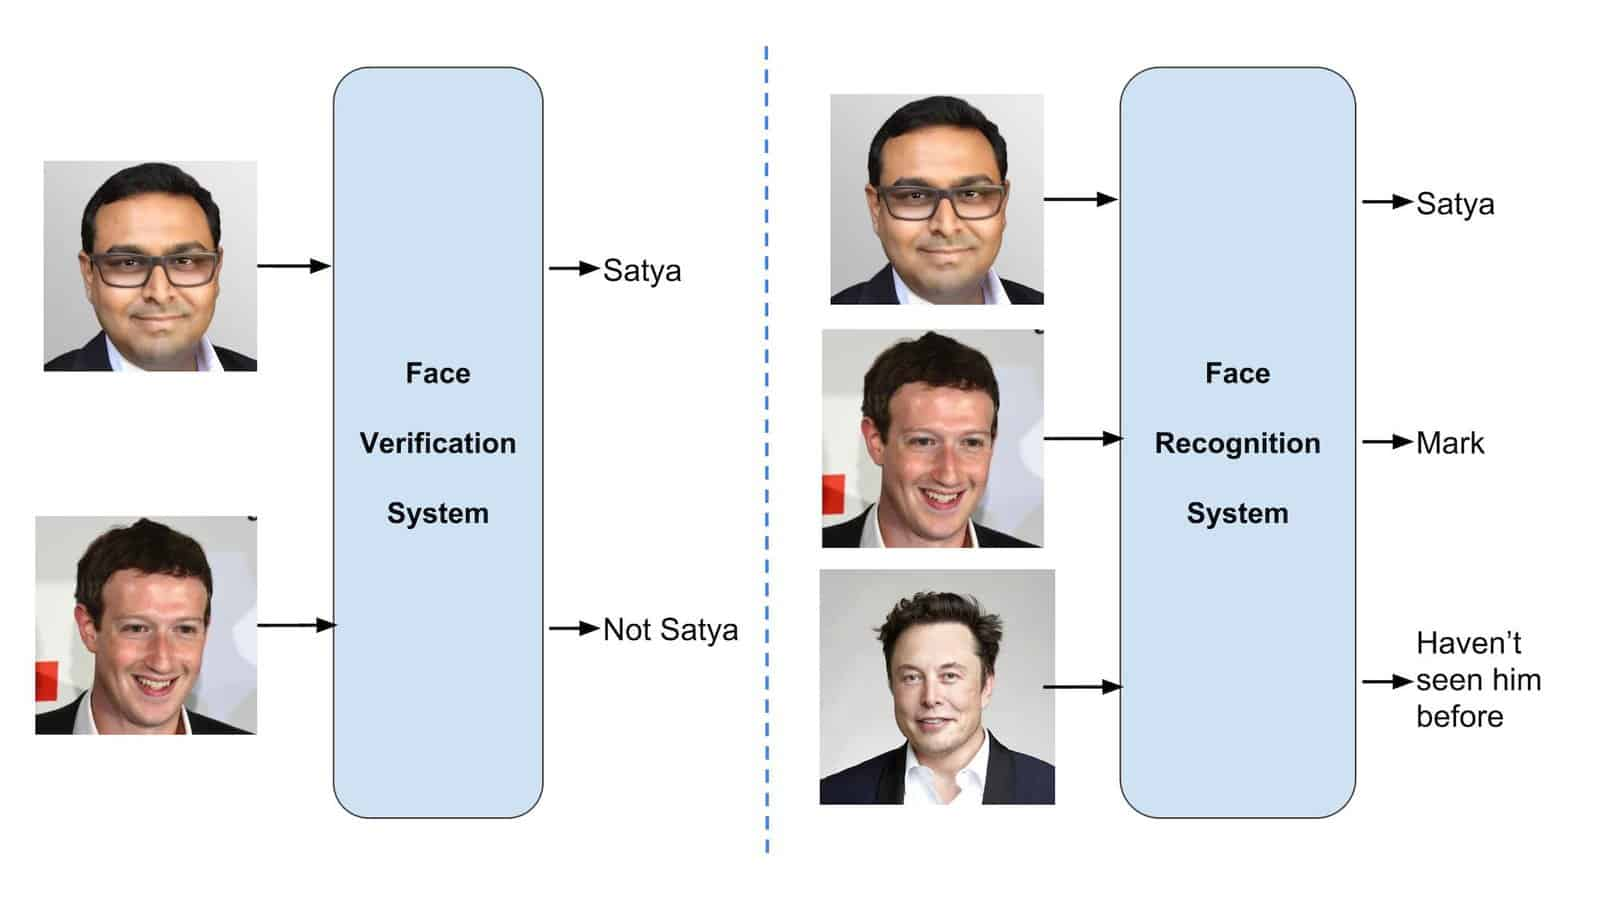
\includegraphics[width=.68\textwidth]{images/face_verification_identification}}
		\caption{Diferencia entre verificación e identificación de rostros.}
		\label{fig:Diferencia entre verificación e identificación de rostros}
	\end{center}
\end{figure}




